\documentclass[border=0.25cm]{standalone}
\usepackage{tikz}
\usetikzlibrary{calc}
\begin{document}

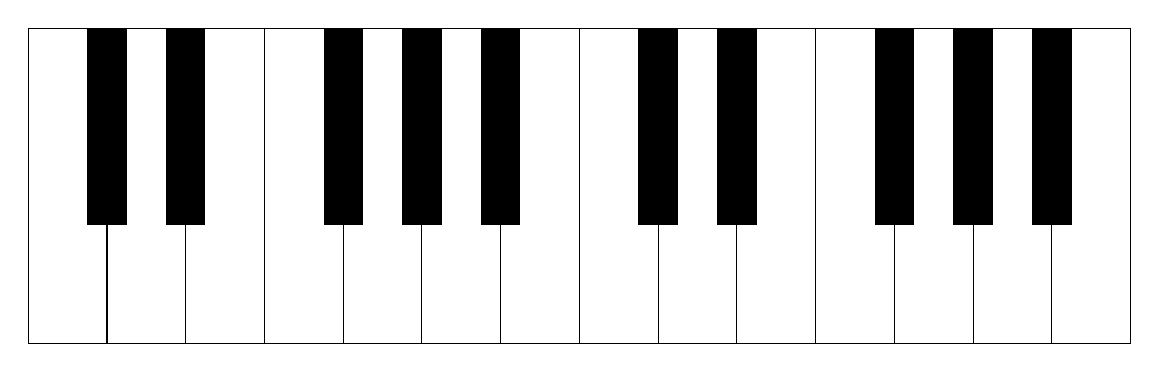
\begin{tikzpicture}

\coordinate (origin) at (0,0);
\coordinate (stave) at (origin);
% left line of first key
\draw (0.25,-1) -- (0.25,-5);

\newif\ifblacknote
\foreach \octave in {0,...,1}
    \foreach \pitch [count=\p] in {C, D, E, F, G, A, B}{
        % calculate x position from octave and pitch
        \pgfmathparse{\octave*7+\p+0.25}
        \edef\myx{\pgfmathresult}
        % draw three lines for top, right, bottom of this key
        \draw (\myx,-1) -- (\myx,-5);
        \draw (\myx,-1) -- ($(\myx,-1)+(-1,0)$);
        \draw (\myx,-5) -- ($(\myx,-5)+(-1,0)$);
        \blacknotefalse
        \ifcase\p
        \or
            \blacknotetrue
        \or
            \blacknotetrue
        \or
        \or
            \blacknotetrue
        \or
            \blacknotetrue
        \or
            \blacknotetrue
        \or
        \else
        \fi
        \ifblacknote
            % recalculate x
            \pgfmathparse{\octave*7+\p}
            \fill ([xshift=0.25cm, yshift=-1cm]stave.south -| \pgfmathresult,0) ++(-0.25cm,0) rectangle ++(0.5cm,-2.5cm);
        \fi
    }

\end{tikzpicture}
\end{document}